\documentclass{article}

\usepackage[main=english,vietnamese]{babel}
\usepackage[T1]{fontenc}
\usepackage[utf8]{inputenc}
\usepackage[sexy]{evan}
\usepackage{matchsticks}
\usepackage{wrapfig}
\usepackage{listings}

\newtheorem{hint}{Hint}

\title{The Extremal Principle}
\author{Nghia Doan}
\date{\today}

\begin{document}

\maketitle

In this article, we discuss the Extremal Principle and its applications.
One of the simplest forms of the principle is as follow:
"in a finite set of numbers, there is a number with minimal value,
i.e. it is smaller than or equal to any other number in the set.
Similarly there is a number with maximal value,
i.e. it is larger than or equal to any other number in the set."

\textit{Proof by contradiction} is an extremely useful tool when combining with the Extremal Principle,
as you will see in below examples.

\begin{example*}[Dancing at a party]

    At a party no boy danced with all the girls,
    but each girl dances with at least one boy.
    Prove that there are two pairs of girl-boy $(g_1, b_1)$ and $(g_2, b_2)$
    who danced with each other but $g_1$ did not dance with $b_2$
    and $g_2$ did not dance with $b_1.$
\end{example*}

\begin{soln}
    Let $b_1$ be \textit{the boy who danced with the maximum number of girls.}
    Then there is a girl $g_2$ who he did not danced with.
    For $g_2$ there is a boy $b_2$ that $(g_2,b_2)$ danced together.
    Among the girls who danced with $b_1$ there is at least one $g_1$ who did not danced with $b_2,$
    otherwise $b_2$ danced with $g_2$ and all the girls that $b_1$ danced with,
    meaning $b_2$ danced with more girls than $b_1,$ contradicting with the choice of $b_1.$
\end{soln}

\begin{example*}[Infinity by contradiction]

    $\Omega$ is a set of points on the plane.
    Every point in $\Omega$ is a midpoint of two points in $\Omega$.
    Show that $\Omega$ is infinite set.
\end{example*}

\begin{soln}
    Suppose that $\Omega$ is a finite set.
    According to the Extremal Principle,
    \textit{there exists two points $A, B \in \Omega,$ such that the distance $AB$ is maximal.}

    Now, since $B \in \Omega,$ there exist two points $C,D \in \Omega$ so that $B$ is the midpoint of $CD.$
    \begin{center}[h]
        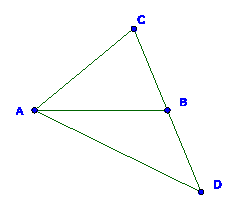
\includegraphics[width=3cm]{./svg/pdf/2022-2-ms-1-3.pdf}
    \end{center}        

    Since one of the angles $\angle ABC,$ $\angle ABD,$ says $\angle ABD$ is at least $90^{\circ},$
    thus in $\triangle ABD,$ $AD > AB.$
    This contradicts the assumption that $A, B$ are the two points in $\Omega,$ such that the distance $AB$ is maximal.

    Thus, there are no such two points $A, B,$ so \framebox{$\Omega$ is infinite set.}
\end{soln}

\newpage

\begin{example*}[How many olives did the knights eat?]

    At the dinner of King Anthony, several knights sits around a round table eating green olives.
    Minh, the Magician, made sure that each knight ate either twice as many olives
    or $10$ olives less than his right neighbour. 
    Is that possible that the knights could have eaten exactly $1001$ olives?
\end{example*}

\begin{soln}
    Let assume that the knights have eaten exactly $1001$ olives.
    Let choose the knight who \textit{ate the smallest number of olives}.
    (If there are some of them, choose one.)
    His neighbour on the left, knight $k$, ate either $10$ less or twice more.
    Since the knight we chose ate the smallest number of olives, then knight $k$ ate twice as many.
    Therefore, knight $k$ ate an even number of olives. 

    The neighbour on the left of knight $k$ ate either twice as many olives or $10$ olives less,
    hence he ate an even number of olives as well. Making the full circle, we'll end us with the first knight,
    who must have eaten an even number of olives as well.
    
    Therefore, the total number of olives must be an even number.
    The number of olives eaten \framebox{cannot be $1001.$}
\end{soln}

\begin{example*}[Chop the flies]

    $25$ flies are resting on the outdoor table in the garden, waiting for lunch to be served.
    It is known that for any three of them, two are at a distance less than $20$ cm;
    and there are at least a pair of flies that are further than $20$ cm from each other.
    
    Minh's mother gave him a fly swatter, shown below, with a hoop of radius $20$ cm,
    With a single strike he can swat the flies where the hoop landed.
    In \textit{at least} how many strikes can he swat all of them?
    \textit{Note that Minh is so fast that the flies do not have time for reaction during and between his lightning strikes.}
\end{example*}

\begin{soln}
    If no $2$ flies are further than $20$ cm from each other,
    Minh can strike them all in $1$ strike by aiming the center of the swatter at any fly. 
    But this is not the case, so let’s assume there are $2$ flies, $A$ and $B$, that are more than $20$ cm apart.
    Then, every other fly is either in a $20$ cm radius of $A$ or in a $20$ cm radius of $B.$
    Out of the $23$ remaining flies either at least $12$ will be in the $20$ cm radius of $A$
    or $12$ will be in the $20$ cm radius of $B$.
    Swatting that the $A$ or $B$ fly with the center of the swatter kills at least $13$.

    Thus, by \framebox{$2$} strikes, he can swat them all.
\end{soln}

\end{document}